% %
% LAYOUT_E.TEX - Short description of REFMAN.CLS
%                                       99-03-20
%
%  Updated for REFMAN.CLS (LaTeX2e)
%
\documentclass[twoside,a4paper]{refart}
\usepackage{makeidx}
\usepackage{ifthen}
\usepackage{graphicx}
\usepackage{listings}
\usepackage{color}
\lstset{language=R,
	basicstyle=\footnotesize,
	stringstyle=\color{red},
	keywordstyle=\color{blue},
	rulecolor=\color{black}
} 
% ifthen wird vom Bild von N.Beebe gebraucht!

\def\bs{\char'134 } % backslash in \tt font.
\newcommand{\ie}{i.\,e.,}
\newcommand{\eg}{e.\,g..}
\DeclareRobustCommand\cs[1]{\texttt{\char`\\#1}}

\title{Validate: A Workflow for Evaluating Performance for GWAS/QTL Tools Using Known-Truth Datasets}
\author{Ann Stapleton, Kurt Michels, and Dustin Landers \\
University of North Carolina Wilmington \\
}

\date{}
\emergencystretch1em  %

\pagestyle{myfootings}
\markboth{Validate: A Workflow for Evaluating GWAS/QTL Tools}%
         {Validate: A Workflow for Evaluating GWAS/QTL Tools}

\makeindex 

\setcounter{tocdepth}{2}

\begin{document}

\maketitle

\begin{abstract}
        Understanding the effectiveness of Genome-Wide Association (GWAS) and Quantitative Trait Loci (QTL) analytical tools under various situations is crucial to deciding which tools are best given a particular problem. Validate provides a way to return classification and regression performance measures for large amounts of tool outputs generated using known-truth simulations. We also provide solutions for aggregating hundreds or thousands of outputs in to a single folder on the iPlant data store, so that Validate can be used.\end{abstract}

\tableofcontents

\newpage

%%%%%%%%%%%%%%%%%%%%%%%%%%%%%%%%%%%%%%%%%%%%%%%%%%%%%%%%%%%%%%%%%%%%

\begin{center}
	\makebox[12cm][r]{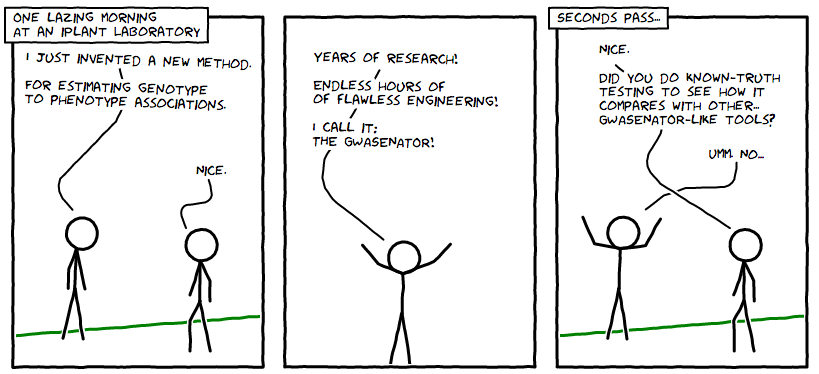
\includegraphics[width=17cm]{doc_comic1}}
\end{center}

\section{Introduction}

\subsection{About the Developers}

\marginlabel{Project Lead and Principal Investigator}Dr. Ann Stapleton works at the interfaces, such as the junctions between research and teaching, individual research projects and large collaborative projects, the organization of international meetings and high-school teacher inquiry labs. Most recently, she has worked at the interface between plant biology and software engineering, leading the way to broad methods applicable to evaluating genotype-to-phenotype analytical methods.

\marginlabel{Statistical Analyst and Developer}Dustin Landers received a BS from Appalachian State where he learned a lot about survey research and using statistics to solve problems and answer questions. He continued his education at UNCW by studying Applied Statistics. Moving from world of polling and survey statistics to the that of Big Data, he has an interest in bridging the gap between statistics and software engineering and seeing the combined discipline brought to bear on problems once considered impossible.

\index{author}

\subsection{Why Validate?}

To test known-truth data sets, we originally weren't sure of the best way to approach the problem. We had the idea of using ROC plots. We wanted to look at true positive rates, false positive rates and accuracy. Of course, this was never really feasible because any one simulation run could be atypical, and all of these methods could only analyze a single simulation run. We asked ourselves how could we run lots of simulations through a tool, and test the outputs in a way that gave us insight in to the performance of these GWAS and QTL tools?

We decided that in order to allow lots of simulations to be tested, we needed a method that that allowed iterations over hundreds or even thousands of simulation-runs. This birthed the idea of Validate, which is a tool that returns these sorts of measures of tool success for massive amounts of outputs.

But how do we run all these simulations? How do we store them all in a single location so we can calculate these measures? How do we visualize them?

These are the problems we sought to solve. For each problem, we have our own solution. We also left them divided. This way you can decide whether to use our solution or to use your own if you have a unique scenario.

\subsection{Getting iPlant Credentials}

\subsection{Getting Your Application on an API}

\subsection{Where Can I Get These?}

\subsection{How to Use This Manual}

Evaluating a GWAS/QTL tool with Validate is essentially four major steps after your application is installed on either the iPlant Foundation API or the Agave API:
\begin{enumerate}
\item \textbf{Running the Tool With Simulations As Inputs.}
\seealso{Section 2}
This step involves deciding what simulations to use and then iterating over those simulations and submitting them as job requests through the API. We recommend using some sort of scripting method that you are comfortable with. At this point, we don't have a standalone application for submitting jobs. We use rPlant, which is freely available R package that allows you to connect with iPlant's API layer to submit job requests.
\item \textbf{Aggregating the Outputs into a Single Folder.}
\seealso{Section 3}
This part is a bit of a logistical exercise. You need to put all the tool outputs (from Step 1) that you want to be analyzed using the same known-truth metadata in to aggregate folders. For example, say we are using simulations that are generated using varying levels of heritability. Since the varying heritability values in essence produce different SNP effects, we need to essentially run Validate three separate times. Validate requires an input on an entire folder, and then iterates over those tool outputs. So the first step here, is to decide how many different runs we need to do and then create that many folders. We provide a GUI tool, \textit{Aggregate} that allows you to select files from multiple folders on your iPlant data store (multiple runs of a single tool) and move those (or aggregate them) in to a single folder.
\item \textbf{Running \textit{Validate} on the Aggregated Folder.}
\seealso{Section 4}
Once you have all your outputs in aggregated folders. You can simply log in to the iPlant Discovery Environment and run \textit{Validate} on that folder. You must have at least two columns with header names in the outputs: The name of the SNP column, and the name of threshold column (such as P-value). Further, if you wish the get back effect size estimation errors, you must also know the column on the estimated effect size column (for example, PLINK's is BETA). Text files with known SNPs and effect sizes must also be included. Once you submit Validate, you will receive a notification when it is completed. The \textit{Validate} output will be columns of performance measures for each tool output.
\vspace{-1.3mm}
\item \textbf{Running \textit{Demonstrate} on the Validate Output.}
\seealso{Section 5}
Finally, once you have outputs from \textit{Validate} (which may be more than one), you need to combine them and test the differences in your measures between your simulation's parameters. Demonstrate is an R package (to be installed on the iPlant DE) that quickly combines all your results files in a folder you specify and returns sciplot factorial graphs for parameters you specify. It also returns the combined results file so that you can perform your own analyses.
\end{enumerate}

\newpage
\section{Running Simulations}

%\index{layout design}

\subsection{How To Run Simulations with rPlant}

\textbf{Step 1-A) Install R and rPlant}

We will first show you how to batch run simulations with rPlant. First, we are using the latest R version, 3.0.2. When you open the R console, it should look something like this (we are using a Mac, so yours may look slightly different, but it will function essentially the same).
\begin{center}
	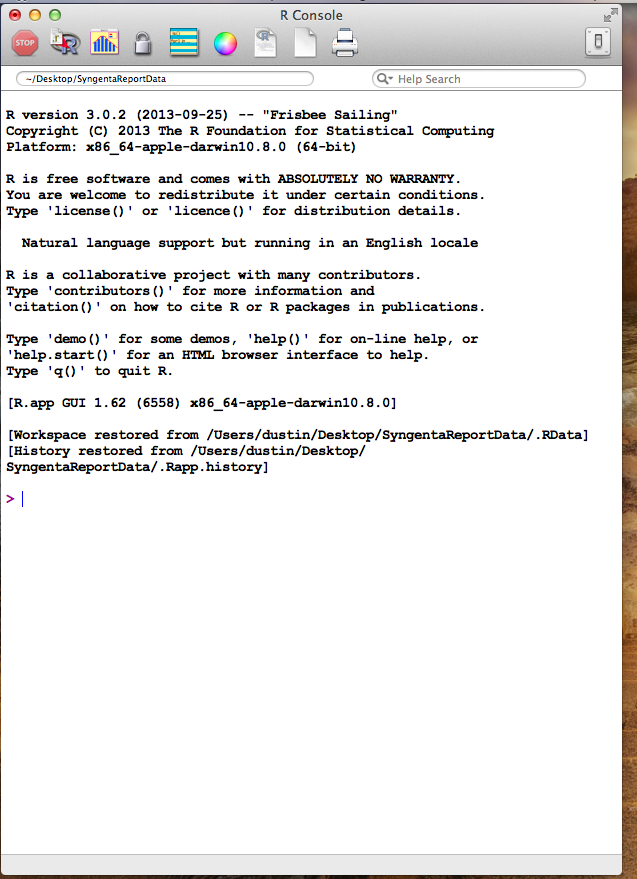
\includegraphics[width=\textwidth]{doc_step1_1}
\end{center}

If you haven't already installed rPlant, we recommend that you do that. After that, you need to validate your iPlant credentials so that you can access your simulation files. Then, you will need to get a list of the names of your simulations files and iterate over them in a for loop, submitting jobs to your installed application. 

\textbf{Step 1-B) Consider the strategy you want to use. Do you want to use all your known-truth data sets, or just a sample? And if a sample, should you take a stratified sample?}

The following code is to just an example of how the submission may go assuming your known-truth data sets are in something like a raw format, where each known-truth data set is stored in a single file. rPlant assumes you already include your iPlant data store username in the files path, so that "iplant/home/username/simulations" is just written as "simulations" or "iplant/home/username/analyses" is just written as "analyses". This is, of course, because validating your credentials allows you to not have to keep typing you user information over and over again. \seealso{These are mainly just example codes. Although you are welcome to copy ours.}


%\begin{center}
\begin{lstlisting}[frame=single]
> install.packages("rPlant")
> require(rPlant)
> Validate("username", "password")
> mydir <- ListDir("simulations")
> for (i in 1:nrow(mydir)) {
+	SubmitJob(job.name=NULL,
	application="myGWASapplication", 
+	file.path="simulations", file.list=list(mydir[i,1]))
+	print(i)
+ }
\end{lstlisting} 
%\end{center}

\textbf{Step 1-C) Find out the name of your application on the API, and the inputs required.} 

\vspace{-1mm}

You need to make sure of the specific application name assigned to your tool in the API and of any special parameters or inputs required in order to run. For example, PLINK requires a PEDMAP format. The PEDMAP format is essentially two files, the .PED and the .MAP file for each known-truth data set. 

For example, our simulation files are stored in a shared folder, where each odd file number is a .PED and each even is a .MAP. Each odd is a .PED file and the subsequent file number is a .MAP like so:
\begin{center}
	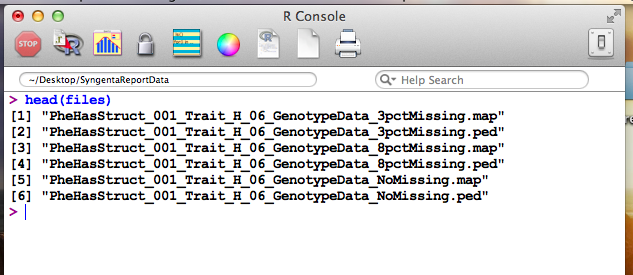
\includegraphics[width=\textwidth]{doc_step1_2}
\end{center}

As can be seen, for our particular structure we would need to submit two files for each run. So let's walk through it. We first can list all the apps in order to find ours (which we have already installed), so that we can get the exact name that we need to use for the SubmitJob function.

\begin{center}
\begin{lstlisting}[frame=single]
> ListApps()
\end{lstlisting}
\end{center}

\begin{center}
	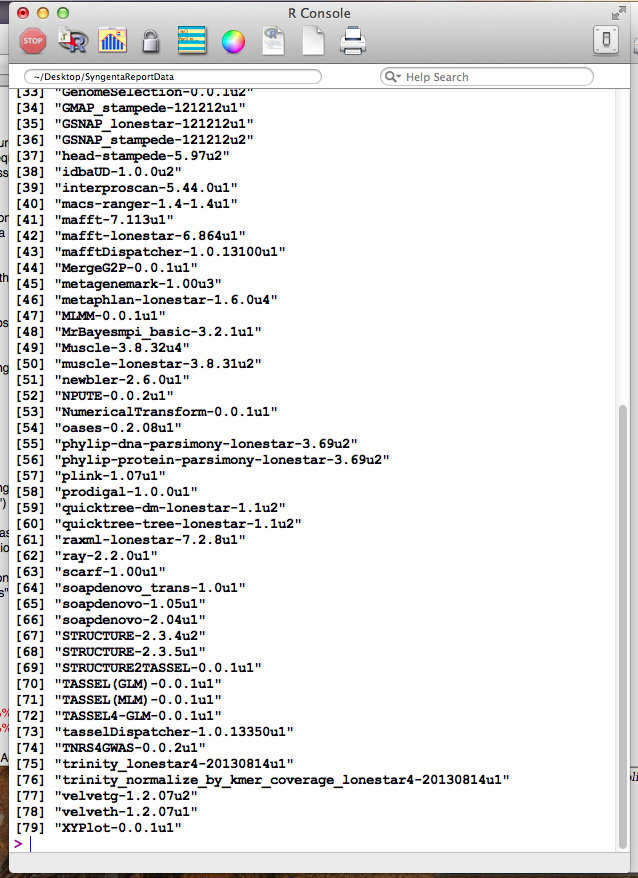
\includegraphics[width=\textwidth]{doc_step1_3}
\end{center}

We can see that the exact name of PLINK on the Foundation API is "plink-1.07ul". We will revisit the earlier explanation to see how we would submit a PLINK job using the PEDMAP format.

\textbf{Step 1-D) Use the short R script to select known-truth data sets and submit a job run for each one using your application.}

\begin{center}
\begin{lstlisting}[frame=single]
> install.packages("rPlant")
> require(rPlant)
> Validate("username", "password")
> mydir <- ListDir("simulations")
> for (i in 1:nrow(mydir)) {
+	SubmitJob(job.name=NULL, 
	application="plink-1.07ul", 
+	file.path="simulations", file.list=list(mydir[i,1], 
+		mydir[i+1,1]))
+	print(i)
+ }
\end{lstlisting}
\end{center}

This should iterate over each simulation in our data set and submit a PLINK job to the iPlant hardware. Since iPlant uses a queuing system, this effectively distributes your workload over many computer nodes as needed. This is obviously helpful in achieving a high volume of runs, even outside of known-truth testing. Now you know how!

\subsection{Using rPlant to Sample From Your Known-Truth Data Sets}

Let's say, for example, that we had 600 total known-truth data sets: Our known-truth datasets are generated from hundred different genotypes, with three different types of simulated missing values such as 0\%, 3\%, and 8\%. In addition, we have data generated with and without population structure (meaning the stochastic processes generated the data have either a single population mean or varying group means). 

Say that we didn't want to run all of them, but maybe just half of them. In many cases, you may have substantially more than 600 and thus sampling makes much more sense then it does in this example. 

We can use some scripting in R and rPlant to accomplish the same thing we did earlier but with some random sampling. Here is the code we used to sample 300 known-truth PEDMAPs for PLINK.

\begin{center}
\begin{lstlisting}[frame=single]
> set.seed()
> require(rPlant) 
> Validate("username", "password")
> mydir <- ListDir("simulations")
> genos <- matrix(nrow=1200,ncol=1)
> break.data <- function(x,y=2) {
+	broken <- unlist(strsplit(x,'_',TRUE))
+	return(broken[y])
+ }
> mydir <- mydir[,1]
> for (i in 1:length(mydir)) {
+	genos[i] <- break.data(files[i],2) 
+	gens <- na.omit(unique(genos))
+ }
> oddsamp <- seq(1,11,2)
> totest <- list()
> for (i in 1:length(genoa)) {
+	myfiles <- list()
+	for (j in 1:length(files)) {
+		if (breakdat(files[j],2)==genos[i]) {
+			myfiles <- append(myfiles,files[j])
+		}
+	}
>	myfiles <- myfiles[sample(oddsamp,2,FALSE)]
>	myfiles <- unlist(myfiles)
>	for (k in 1:length(files)) {
+		for (p in 1:length(myfiles)) {
+			if (files[k]==myfiles[p]) {
+				totest <- append(totest,k)
+			}
+		}
+	}
+ }
> totest <- unlist(totest)
> for (i in 1:length(totest)) {
+	SubmitJob(job.name=NULL, 
		application="plink-1.07ul", file.list=
+		list(files[totest[i]], files[totest[i]+1]), 
+		file.path="simulations")
+	print(i)
+ }
\end{lstlisting}
\end{center}

Every situation is unique in this case, which is part of the reason we have yet to develop a graphical user interface method for submitting jobs. All that we did in the code above, is demonstrate how rPlant may be used to break up some files that had naming conventions that were separated by underscores. If you look back to the earlier image that showed what our known-truth data sets looked like, you would see that phenotype, heritability information, and population structure are all in the naming format for each data set. 

This is an important piece of information, because without an appropriate naming structure, there would be no way for us to keep metadata on the known-truth data sets throughout this testing process.

We break up the names to grab the pieces about phenotype information in order to essentially stratify-sample our data sets by genotype. We then have six data sets for any one genotype (three missing values types and two population structure types), and then we just pick two at random. 

This insures that we include all of our genotypes in our runs, but there are simpler ways to do this, that basically just random sample from all of our data sets. The following code again assumes you are using PEDMAPs to run PLINK, but that you just want to sample a random 300 (as opposed to a stratified-random sample). 

\begin{center}
\begin{lstlisting}[frame=single]
> set.seed()
> require(rPlant) 
> Validate("username", "password")
> mydir <- ListDir("simulations")
> mydir <- mydir[,1]
> oddsamp <- seq(1,599,2)
> totest <- sample(oddsamp, 300, FALSE)
> for (i in 1:length(totest)) {
+ 	SubmitJob(job.name=NULL, 
+		application="plink-1.07ul", file.list=
+		list(mydir[totest[i]], mydir[totest[i] + 1],
+		file.path="simulation"
+ }
\end{lstlisting}
\end{center}

%\index{rules}

%%%%%%%%%%%%%%%%%%%%%%%%%%%%%%%%%%%%%%%%%%%%%%%%%%%%%%%%%%%%%%%%%%%%%%
%\vspace{-30mm}
\section{Aggregating with Aggregate}
%\label{layout}

\subsection{How to Use the GUI Aggregate Tool}
The second major step is accomplished once all the runs have finished. In our example, depending on the resources available, PLINK can finish in a range from ten seconds to two and half minutes per run (not including the queuing process). This is non-linear as well, because many will be running simultaneously on separate nodes while some remain in queues. Its hard to gauge exactly how long your tool will take, but it will almost definitely run faster on multiple nodes this way.

\textbf{Step 2-A) Log in to the DE and make sure all runs are complete.}

Let's say that we have already run all of our runs. Then we would want to log in to the iPlant Discovery Environment to make sure all the folders are in our analyses folder. As can be seen, each run of PLINK with each distinct known-truth data set has been put in to each folder. If we were to open up each folder, we would see a set of files, of which only one we will want to put through Validate. In the case of this PLINK run, you need to put each file ending in .qassoc (the standard PLINK output filetype) in to a single folder, so that we can run Validate on that folder. 

\newpage
\begin{center}
	\makebox[12cm][r]{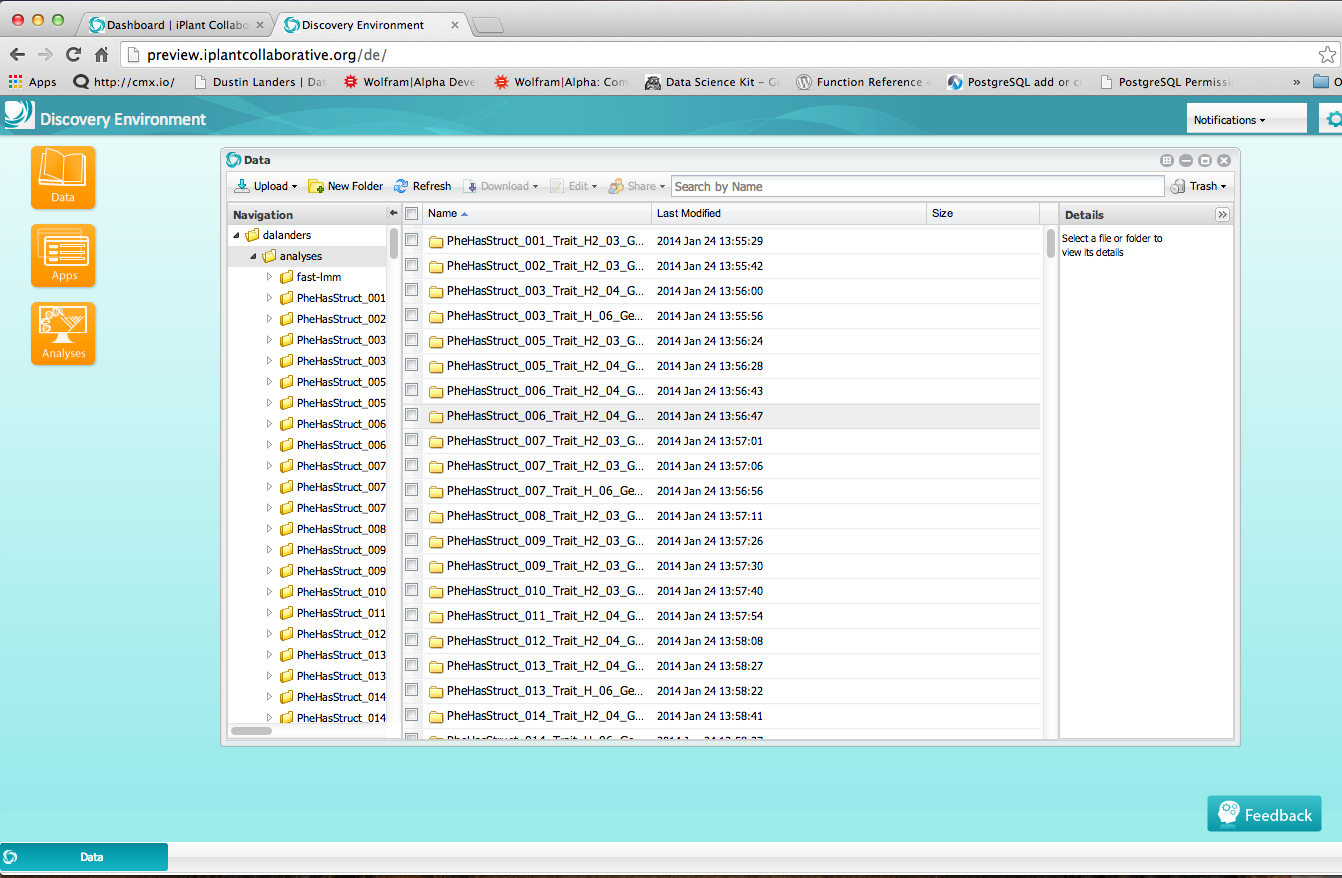
\includegraphics[width=17cm]{doc_step2_1}}
\end{center}

\textbf{Step 2-B) In the DE, create a new folder for your Validate analysis.}\seealso{If you are testing for effect sizes that are different for different levels of heritability, you may want to create more folders in this step. Actually, for the rest of this process, you would have to everything multiple times for each folder you create here. Say for example, I'm testing three different heritability levels, which will have three different groups of actual effects. Then I would need to run Validate three different times, and thus need to make three folders in this step and separate them that way.}

The \textit{.qassoc} files in this case, are the files containing the actual analysis that we will use for evaluating the effectiveness of PLINK. Particularly, those are the predicted values for each SNP based on the PLINK algorithm. Now, it's time to compare those predicted values with what we know to be the actual values. 

You need to create a folder that we will use for our Validate analysis. In the DE, create a folder called \textit{my\_Validate\_analysis}. 

The goal is to look inside each of the 300 folders we created, and pull out the \textit{.qassoc} file and move it to the folder marked \textit{my\_Validate\_analysis}. 

Since this would take hours, we suggest you launch the application we created called \textit{Aggregate} that provides a fairly easy way to do this (at least, comparatively easier). 

\textbf{Step 2-C) Launch Aggregate.} \seealso{Note that in rPlant, your don't have to type your username and you begin iPlant data store file locations immediately. For example, in rPlant, the same location would just be written as "analyses"} 

Once you launched \textit{Aggregate} you will see there is a place to enter your username and password. Go ahead and enter those. 

\textbf{Step 2-D) Enter username and password.}

Now, you need to type the out the full location of the folder starting with username where your analyses are located. In this case, all of our PLINK analyses folders are located in the folder \textit{dalanders/analyses}.

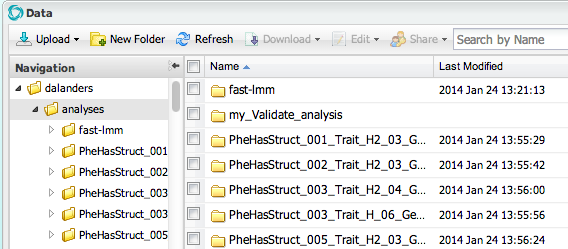
\includegraphics[width=\textwidth]{doc_step2_2}

\textbf{Step 2-E) Enter the folder location where all your tool analyses are located and click \textit{View Folders in Directory}.}

We will enter \textit{dalanders/analyses} and click the button \textit{View Folders in Directory}. This is provide us with a list of all the files and folders in that directory on the iPlant data store in the left-most listbox.
\vspace{-1mm}
\begin{center}
	\makebox[12cm][r]{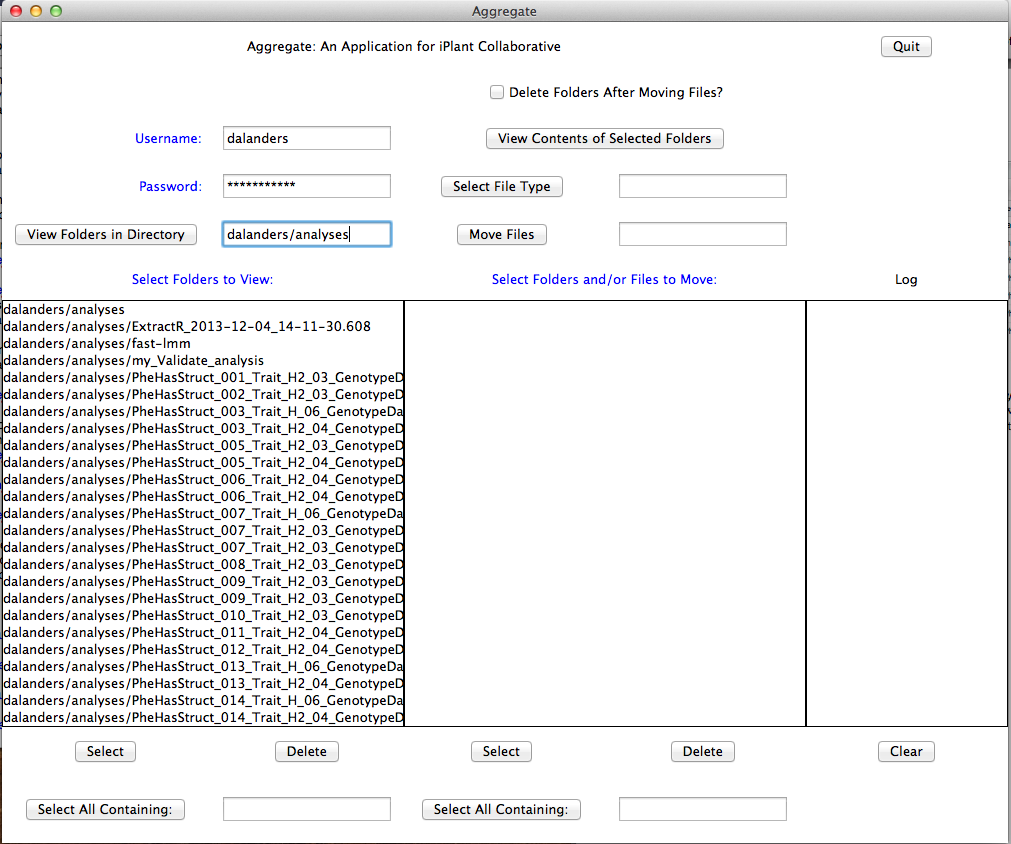
\includegraphics[width=17cm]{doc_step2_3}}
\end{center}

\textbf{Step 2-F) Select only folders from the known-truth data sets runs.}

Now, we want to just select the folders that we just created. You can select them all using Control + Click to select individual ones, or if you wish to just select the whole list you can select all between two files by using Shift + Click. 

We also provide a method selecting many at us by using the \textit{Select All Containing:} logic button at the bottom of the listbox.

For example, our analyses folders all contain the words "GenotypeData" or even "Trait". 

We can type in the box just to the right of \textit{Select All Containing:} "Trait" and then click the button. This should select just the folders we are interesting obtaining the contents of.

We can scroll up and down to make sure that we have only selected the ones that we need. If we have selected a few that we didn't intend to. We can select those using the mouse and then click the \textit{Delete} button to remove those from the list.

\begin{center}
	\makebox[12cm][r]{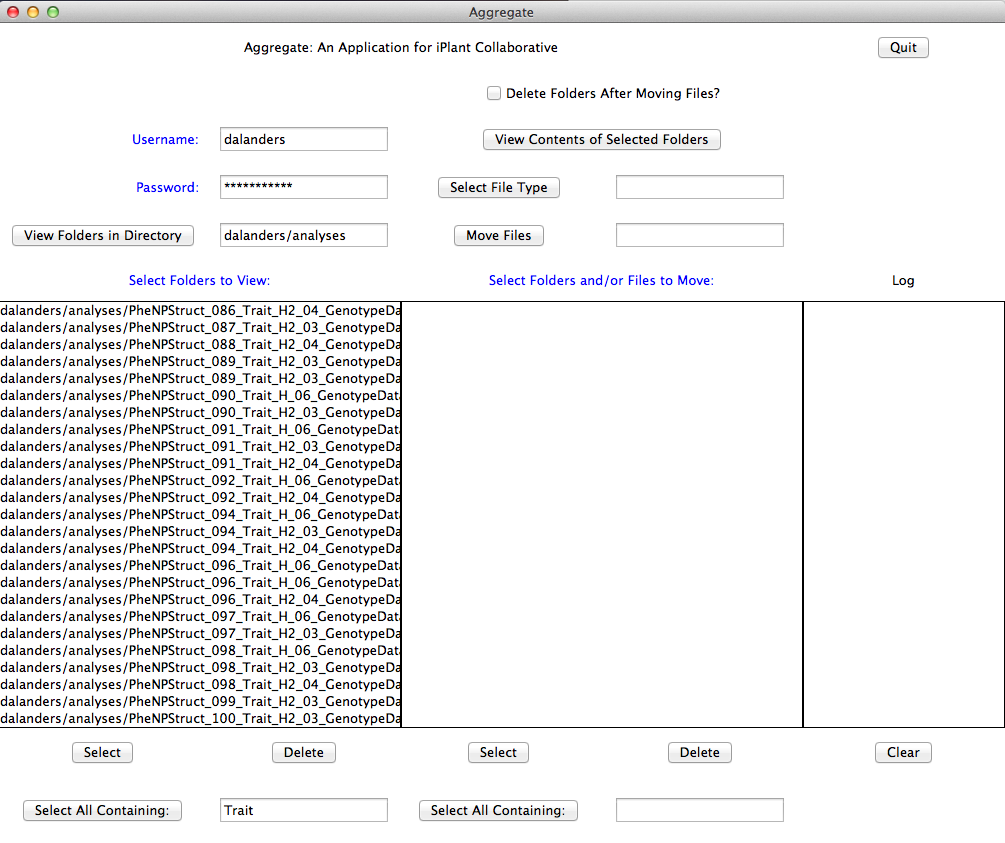
\includegraphics[width=17cm]{doc_step2_4}}
\end{center}

\textbf{Step 2-G) Click \textit{View Contents of Selected Folders}}

Once you've got all your folders in the first listbox, click the button on the right call \textit{View Contents of Selected Folders} and this will iterate over the folders in the left-most listbox and add the contents of all those folders to the right-most listbox. It should take a few minutes, so give it some time. Once its done, see if you can spot the files that you were interested in moving. In our case, they are the files ending in \textit{.qassoc}.

\begin{center}
	\makebox[12cm][r]{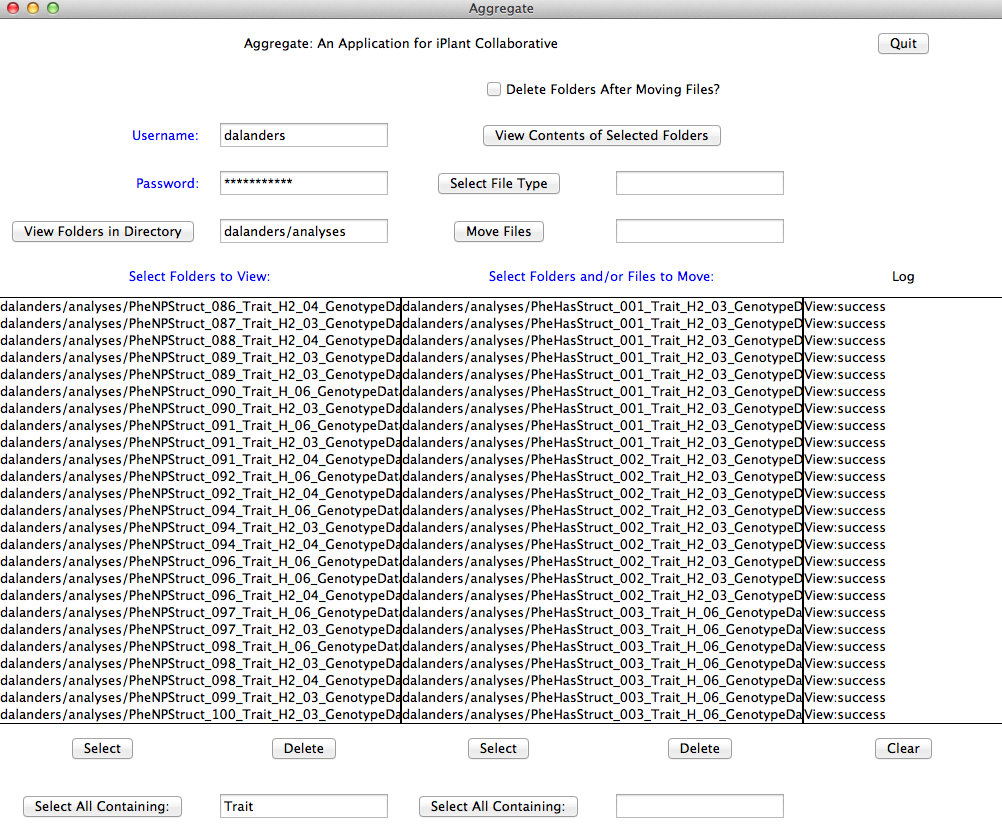
\includegraphics[width=17cm]{doc_step2_5}}
\end{center}

As you can see, every single item in the right-most listbox is a file or folder contained with \textit{one} of the folders in the left-most listbox. Now, we need to select all the files from the right-most listbox that we wish to move to the folder we created in order to run \textit{Validate}.

\textbf{Step 2-H) Select just the tool outputs from the right-most listbox.}

In order to select just the right files that you intend to move, you can use the same \textit{Select All Containing:} logic button we used earlier, or if they all have the same file extension (as ours do with \textit{.qassoc}) then we can use another option.

Above the right-most listbox is a button labelled \textit{Select File Type}. Next to that, we type \textit{qassoc} in and then click the button in order to just select the file types that we want to move.

\begin{center}
	\makebox[12cm][r]{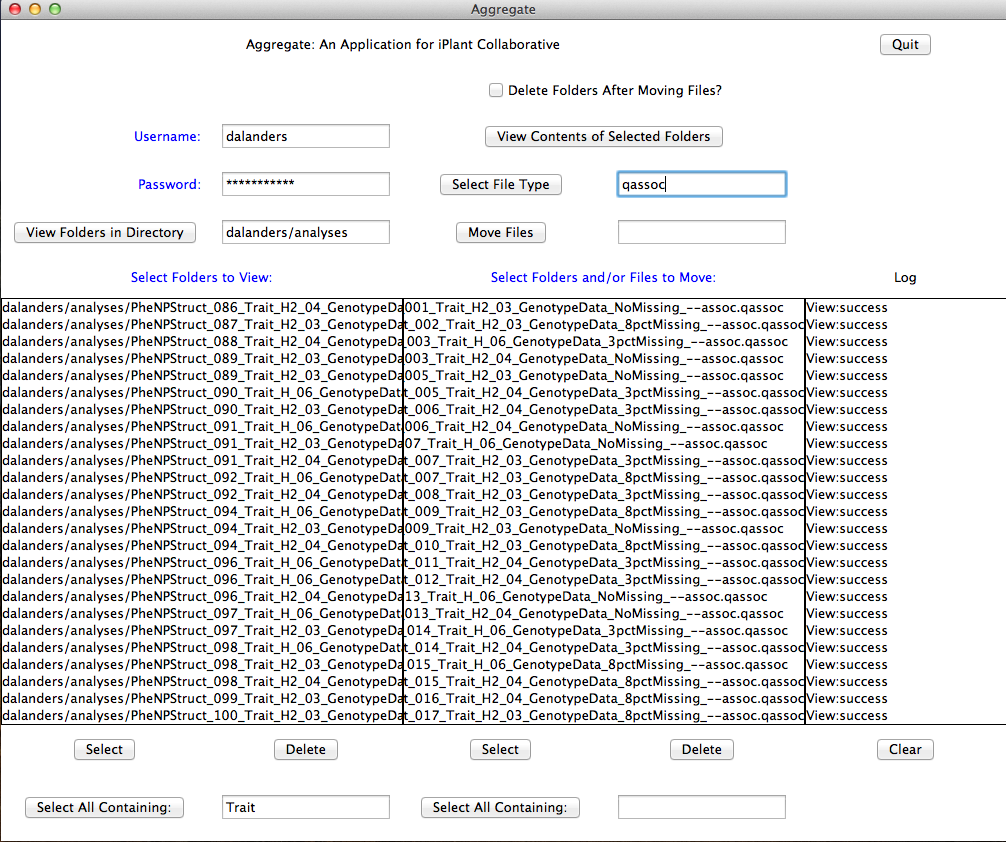
\includegraphics[width=17cm]{doc_step2_6}}
\end{center}

\textbf{Step 2-I) Move the files to your \textit{Validate} analysis folder.}

Now, we can move the files. In the text box next to the \textit{Move Files} button enter the full path of the folder we created just for this purpose in Step 2-B. In our case, we named it \textit{my\_Validate\_analysis} so we would enter in to the text box: \textit{dalanders/analyses/my\_Validate\_analysis}. Then click \textit{Move Files} in order to begin iterating over that list and sending the \textit{.qassoc} files to the folder you created. 

This process can take about as long or longer than it did to actually view the files. Keep in mind, that this process uses the iPlant Foundation API system, so for each item in the right-most list, a request is send to the API to move that file to the folder you specified. 

It may also be worth noting that by the time you read this manual, this could be a fully-integrated step in the iPlant Discovery Environment, as there was talk about this functionality being available given more time. However, we found it necessary, even though this part of the problem is almost entirely logistical, to be able to select files from multiple files and move them in to a single aggregate folder. 

\subsection{How to Use the Aggregate Function in rPlant}

\subsection{How to Use Aggregate on Atmosphere}

\section{Validating with Validate}

\subsection{How to Use Validate on the DE}

\section{Visualizing the Validation}

\subsection{How to Use the Demonstrate R Package}

\subsection{How to Use Demonstrate on the DE}

\subsection{How to Use Demonstrate on Atmosphere}

\section{Acknowledgements}

\section{How to Interpret Performance Measures}

\subsection{AUC}

\subsection{H}

\subsection{KS}

\subsection{TPR}

\subsection{FPR}

\subsection{Accuracy}

\subsection{MAE}

\subsection{RMSE}

hmeasure.net

\end{document}